\documentclass[times, utf8, seminar]{fit}

\usepackage{listings}
\usepackage{longtable}
\usepackage{xcolor}
\usepackage{float}
\usepackage{enumitem}
\usepackage{hyperref}
\usepackage{enumerate}
\usepackage{graphicx}
\usepackage{etoolbox}
\usepackage{datetime}
\usepackage{needspace}
\usepackage[compact]{titlesec}
\usepackage{setspace}
\onehalfspacing

\usepackage[parfill]{parskip}

\begin{document}
\widowpenalty=300
\clubpenalty=300

\lstset{
  language=bash,
  backgroundcolor=\color{gray!25},
  basicstyle=\ttfamily \footnotesize,
  breaklines=true,
  prebreak=\raisebox{0ex}[0ex][0ex] {\ensuremath{\hookleftarrow}},
  columns=fullflexible,
  keywords={},
  mathescape=false
}

\title{Agilni \emph{software development},\newline \emph{Continous Integration (CI)}}

\author{Ernad Husremović}
\brindex{DL 2792}
\verzija {0.9.0}

\mentor{mr. Adil Joldić}

\maketitle

\tableofcontents

%\listoftables
%\listoffigures
\newpage

\begin{abstract}

U ovom radu se na bazi konkretnog primjera\footnote{"HOWTO" stil} prezentuje infrastruktura za kontinuiranu integraciju (CI) 

CI infrastruktura je usko vezana za testnu i SCM\footnote{Source Code management} infrastrukturu\citep{agilegit}

Unutar materijala ćemo obraditi implementaciju \href{http://travis-ci.org}{\color{blue}{''Travis Continous Integration''}} za projekat \href{http://redmine.bring.out.ba/projects/knowhow}{\color{blue}{''F18 knowhow''}}.

Za realizaciju ćemo koristiti sljedeće komponente:
\begin{itemize}
  \item Github servis, F18 knowhowERP repozitorij - \url{https://github.com/knowhow/F18\_knowhow}
  \item Travis CI  \url{https://travis-ci.org}
  \item Vagrant test environment  \url{http://vagrantup.com}
\end{itemize}

\keywords{open source software, OSS, travis, CI, continuous integration, vagrant, github, git}
\end{abstract}

% abstract end

\begin{document}
\chapter{Uvod}

\section{Zašto ''Continuous integration'' ?}

Mnogi softverski projekti imaju skriveno kašnjenje između trenutka kada developerski tim kaže "Gotovi smo" i stvarnog trenutka kada je softwarew spreman za isporuku klijentu\citep[str. 183]{agileart}. Nekada je se to kašnjenje može rastegnuti na mjesece.
Spajanje pojedinih komponenti, kreiranje ''installer''-a, kreiranje inicijalne verzije baze podatataka, kreiranje korisničkog uputstva, itd.
U međuvremenu, kompletan tim je pod stresom, ne uzimajući u obzir činjenicu da će ove "post-development" procedure trajati tako dugo. Takvo stanje redovno generira dodatne greške i kašnjenje.
Kontinuirana integracija (CI) prevenira ovakve situacije. Ona obezbjeđuje da se nakon svakog novog commit-a kreira i testira nova verzija software-a. CI omogućava da se odmah nakon razvojnog ciklusa korisniku može isporučiti nova verzija (produkcija).

\begin{quotation}
\noindent \emph{\large Glavni cilj CI-a je mogućnost isporuke (eng. deployment) projekta korisniku u svako vrijeme.}
\end{quotation}

\section{Travis CI}
''Travis CI'' je slobdan CI sistem za opensource developere. Jedini preduslov je da se sofverski repozitorij koji ''travis'' pokriva nalazi na ''github''-u.

Travis funkcioniše tako što se aktivacijom usluge za određenih github projekat, nakon svakog ''commit''-a keira vagrant box\footnote{Više o vagrantu materijalu ''Agilni software development, test \& deploy''\citep[str. 3]{agiletestdeploy}}. Po kreiranju vagrant box-a, pokreću se komande i vrši konfiguracija box-a u skladu sa konfiguracijskim fajlom \href{https://github.com/knowhow/F18_knowhow/blob/master/.travis.yml}{\color{blue}{.travis.yml}}.

Interesatno je uočiti da je kompletan projekat spoznoriran od više sofverskih vendora koji na principu sponzorstva dodjeljuju dio svoje infrastruktinfrastrukture projektu\footnote{Organizacija projekta je u potpunosti u duhu ''opensource''-a.}

\section{F18 knowhowERP}

F18 je ''client-server'' aplikacija:
\begin{itemize}
    \item klasični ('rich') klijent pisan u programskom jeziku ''harbour'' 
    \item server baza podataka PostgreSQL
\end{itemize}


\subsection{F18 test-case-ovi}

Sa stanovišta CI-a problem F18 kao projekta\footnote{F18 svoje korijene vuče iz devedesetih godina prošlog vijeka, originalno pisan za \href{http://en.wikipedia.org/wiki/Clipper\_(programming\_language)}{Clipper}/DOS okruženje} je nepokrivenost source koda testovima. Takođe ''harbour'' nema tako dobar ''test framework'' kao što je to slučaj sa drugim programskim jezicima\footnote{\url{http://en.wikipedia.org/wiki/List_of_unit_testing_frameworks}}. Međutim, čak i rudimentarni test framework \href{https://github.com/hernad/harbour/tree/master/harbour/utils/hbtest}{\color{blue}{hbtest}} pokazao se dovoljnim za realizaciju F18 ''test case''-ova.

S obzirom da ''F18'' korisnik primarno koristi tastaturu za interakciju sa aplikacijom, na ''hbtest'' je dodan set funkcija koje omogućavaju simulaciju rada korisnika putem tastature \href{https://github.com/knowhow/F18_knowhow/blob/master/test/keystrokes.prg}{\color{blue}{''keystrokes.prg''}}

Uz pomoć ''keystrokes.prg'' napravljeni su sljedeći integracijski testovi:
\begin{itemize}
  \item unos \href{https://github.com/knowhow/F18_knowhow/blob/6938fcd1ca/test/i_sif.prg#L35}{\color{blue}{novih šifri u šifarnik}}
  \item povrat fakture \href{https://github.com/knowhow/F18_knowhow/blob/6938fcd1ca/test/i_fakt.prg#L43}{\color{blue}{99-10-7777}}
  \item \href{https://github.com/knowhow/F18_knowhow/blob/6938fcd1ca/test/i_fakt.prg#L69}{\color{blue}{unos fakture sa dvije stavke}} i njeno \href{https://github.com/knowhow/F18_knowhow/blob/6938fcd1ca/test/i_fakt.prg#L165}{\color{blue}{ažriranje}}
\end{itemize}

Da bi se stekao konačan utisak, pripremljen je video koji prikazuje pokretanje F18 integracijskih testova na testnoj vagrant/virtualbox sesiji:

\href{http://www.youtube.com/watch?v=r1SV7GO0MFY}{\color{red}{F18 integracijski testovi, youtube screencast\footnote{\url{http://www.youtube.com/watch?v=r1SV7GO0MFY}}}}

\section{Princip CI-a}

CI koncept je do kraja jednostavan. CI sistem pokreće skriptu koja definiše uspješnu integraciju sistema. Ta skripta uobičajeno obuhvata dvije faze:
\begin{enumerate}
     \item ''build'' - build sistema
     \item ''test'' - izvođenje testova na sistemu kreiranom u predhdnom koraku
\end{enumerate}

Ukoliko je ovaj proces uspješan, ''build \& test'' skripta vraća izlazni kod 0 (exit code = 0, success). U suprotnom, integracija se smatra neuspješnom.

Ovaj jednostavni koncept - ''succes'' / ''fail'' daje razvojnom timu brzu informaciju o tome da li su nove promjene uzrokovale probleme u sistemu (regresiju određenih funkcija) ili se integracija novog k\^oda realizovala uspješno.

\section{Kvalitet testova}

Jasno je da je kvalitetna baterija testova ključna odrednica CI procesa. Ukoliko je izvorni k\^od slabo ''pokriven'' testovima, rezultati CI sistema (oni koji kažu da je integracija uspješna) se moraju uzeti sa rezervom.


\section{''Technical Debth''}

''Technical debt''\footnote{Doslovni prevod na bosanski bi bio ''tehnički dug''. Smatramo da se radi jasnoće bolje držati engleskog termina.} je količina postojećih loših rješenja u oblasti dizajna i implementacije projekta. Ovo uključuje brze i ''prljave'' korekcije koda (eng. dirty hacks) koje omogućavaju da sistem profunkcioniše, ali ga dugoročno čine ranjivim na greške i teškim za održavanje.
''Technical debt'' je najčešće uzrokovan lošim programerskim praksama. Unutar izvornog koda se primjećuje se kroz ogromne funkcije (metode), puno globalnih varijabli, generalno kroz teško razumljiv k\^od funkcije sa puno ''TODO'' ili ''nisam siguran kako ovo radi ..'' komentara.\citep[str. 41]{agileart} 

\section{''Legacy system'' i CI}

F18 knowhowERP je klasični ''Legacy system''\footnote{\url{http://en.wikipedia.org/wiki/Legacy\_system}} . U vrijeme kada je pravljena većina aplikativnog k\^od-a F18, koncept agilnog software developmenta, te njemu pripadajuće su bile nepoznate.

Zato je za većinu funkcija F18 ne postoje automatizirani testovi. Agilni pristup u ovom slučaju dalje sljedeće preporuke:
\begin{enumerate}
  \item Testove postupno uvoditi u kritične funkcije projekta - one koji se najviše koriste i one čija disfunkcionalnost nanosi najveće probleme korisniku\footnote{''Fiskalne funkcije - štampa na fiskalni uređaj'' su dobar primjer kritične funkcije projekta}
  \item Kada se uoči da je potrebno raditi značajne promjene na dijelovima k\^oda (refactoring), prije promjena napraviti set odgovarajućih testova
\end{enumerate}

Ovakav pristup će obezbjediti da se ''technical debth'' projekta kontinuirano umanjuje.

\chapter{Travis}

\section{\emph{Travis} kao indikator ''zdravlja'' našeg projekta}

Nakon što se ''travis'' uspješno podesi, u \href{https://github.com/knowhow/F18_knowhow/blob/master/README.md}{\color{blue}{README.md}} projekta se dodaje sljedeći k\^od:

\begin{lstlisting}
[![Build Status](https://secure.travis-ci.org/knowhow/F18_knowhow.png?branch=master)](https://travis-ci.org/knowhow/F18_knowhow)
\end{lstlisting}

Koji u slučaju neuspjeha rezultira crvenim:

\begin{figure}[H]
\centering
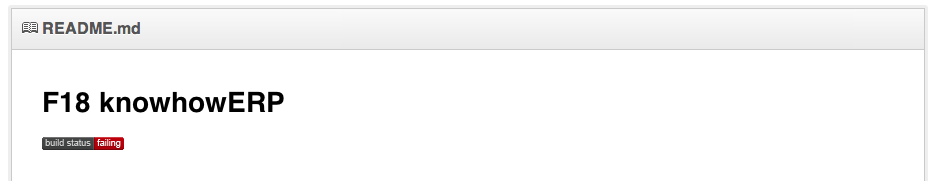
\includegraphics[width=15cm]{img/F18_failing.png}
\caption{travis F18\_knowhowERP build neuspješan - ''failing - red build''}
\end{figure}

A u slučaju uspjepha zelenim statusom:

\begin{figure}[H]
\centering
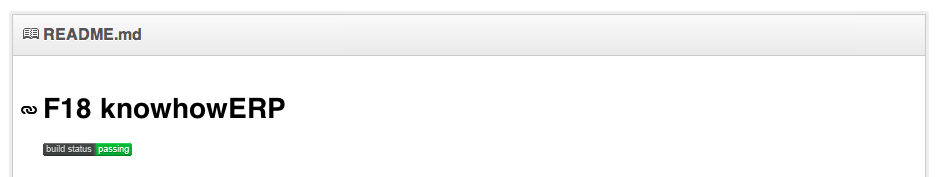
\includegraphics[width=15cm]{img/F18_green.png}
\caption{travis F18\_knowhowERP uspješno - ''green''}
\end{figure}

Travis nam daje detaljne informacije o ''build'' procesu:
\begin{figure}[H]
\centering
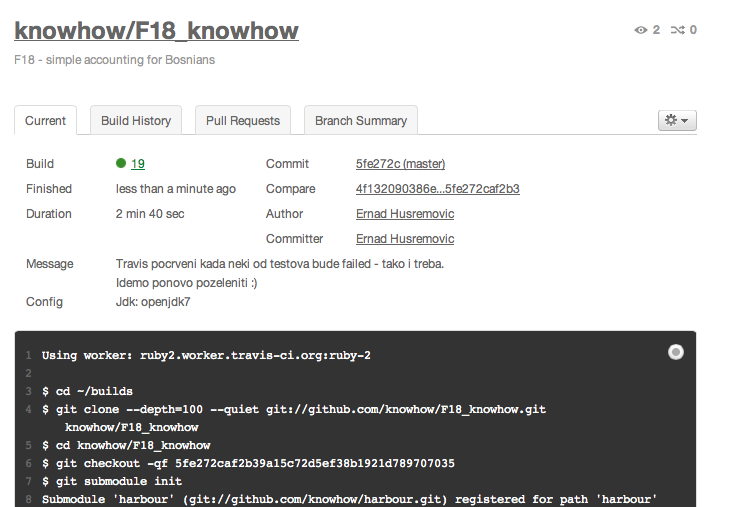
\includegraphics[width=15cm]{img/prvi_green_f18.png}
\caption{travis F18\_knowhowERP prvi uspješan build - ''green build''}
\end{figure}

\section{Travis terminal log}

\subsection{Neuspješno}

Pogledajmo kako izgleda detaljni izvještaja neuspješan build F18:

\begin{figure}[H]
\centering
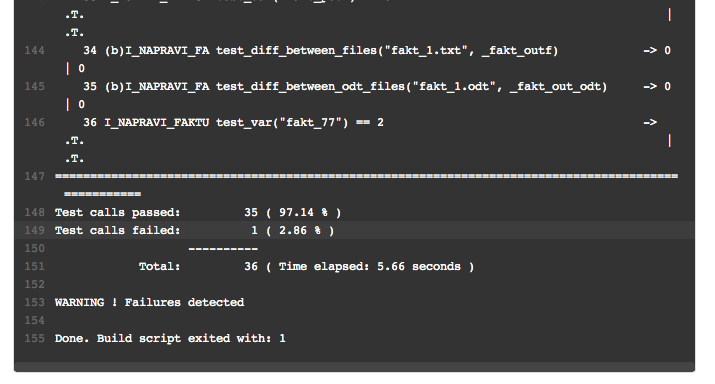
\includegraphics[width=14cm]{img/travis_test_report_failed.png}
\caption{travis F18\_knowhowERP test report - jedan test neuspješan - ''red build''}
\end{figure}

Travis daje prikaz svih operacija na CI sistemu tokom ''build \& test'' procesa.
Na kraju vidimo ''exit code 1'', koji je uzrokovao da ''build'' bude određen neuspješnim.

\subsection{Uspješno}

Uspješni build daje ''exit code 0'':

\begin{figure}[H]
\centering
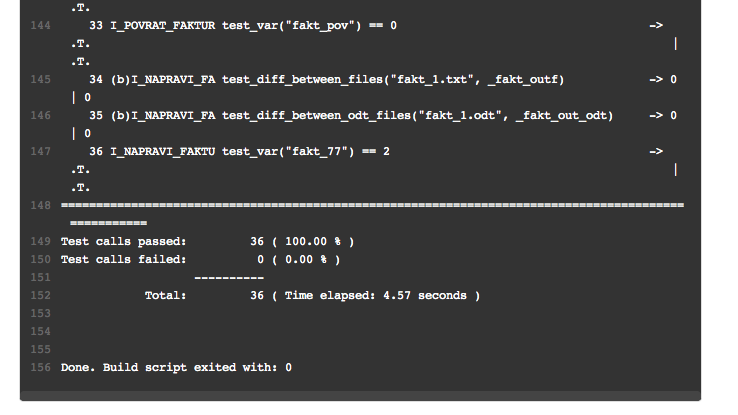
\includegraphics[width=14cm]{img/travis_test_report.png}
\caption{travis F18\_knowhowERP test report prvog uspješnog build-a}
\end{figure}

Od 36 testova koji su pokrenuti, svi su uspješno završili

\section{Email notifikacije}

Trelo, očekivano, ima sistem email notifikacija. Te notifikacije informišu developere o bitnim događajima u ''build'' procesu.

Ono što je za email notifikaciju karakteristično jeste krajnje inteligentan sistem slanja poruka.

Naime, u slučaju uspješnog builda (pod uslovom da je predhodni build bio takođe uspješan) developer ne prima nikakve notifikacije. Tek u slučaju da build ''pukne'' developer počinje primati informacije ''Build failing'', nakon toga ''Still failing''. Kada build ponovo pozeleni, travis prijavljuje "Fixed '". Ukratko, travis se brine o tome da developera ne ''spamira'' nepotrebnim porukama:

\begin{figure}[H]
\centering
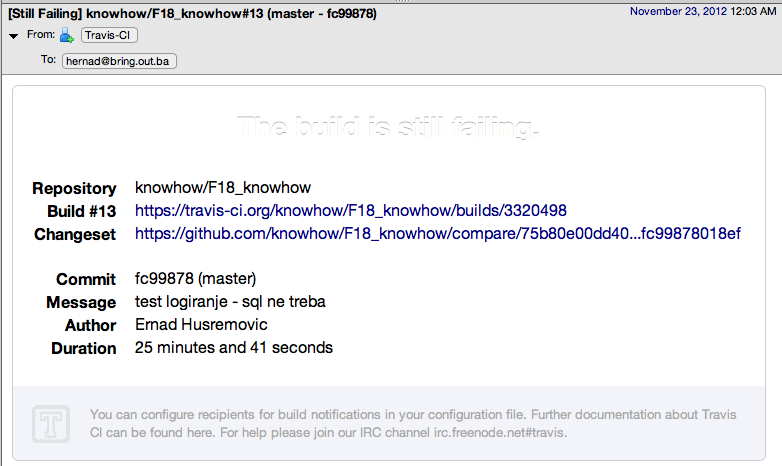
\includegraphics[width=12cm]{img/travis_email_notification.png}
\caption{Travis email notifikacija}
\end{figure}


\chapter{Integracija servisa}

\section{\emph{Github} i \emph{travis}}

Da bi se ''travis'' uopšte koristio, neophodno je da projekat bude hostiran na ''github''-u. Integracija se vrši sistemom Webhook-ova\footnote{\ur{http://en.wikipedia.org/wiki/Webhook}}. U web intefejsu se umjesto ''Webhooks'' koristi termi ''Service hooks''.

\begin{figure}[H]
\centering
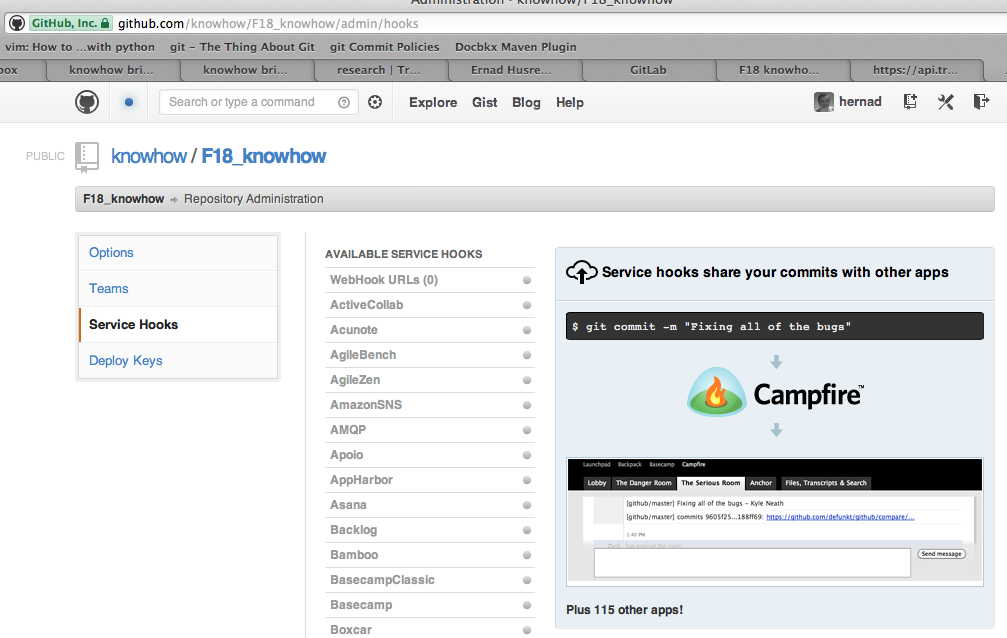
\includegraphics[width=15cm]{img/github_webhook_1.png}
\caption{github web interfejs za podešenja ''Service hook''-ova}
\end{figure}

Github''service hook'' ze podešava unutar travis web interfejsa:

\begin{figure}[H]
\centering
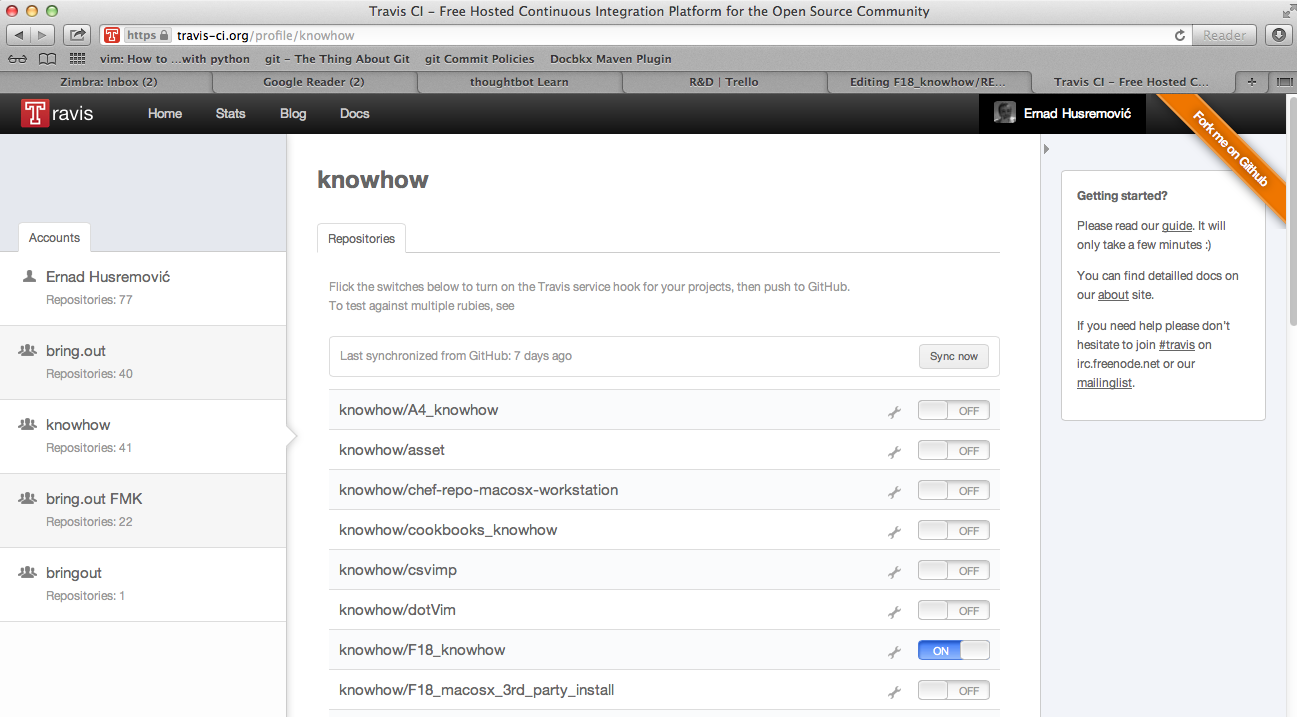
\includegraphics[width=15cm]{img/travis_github_setup.png}
\caption{Travis web interfejs: setup github repozitorija}
\end{figure}

\section{\emph{Github} - \emph{trello} integracija}

Iako ''trello''\footnote{\url{https://trello.com}} kao agilni alat za planiranje strogo gledajući ne pripada tematici ''CI''-a, prikazaće kako se ova integracija realizira:

\begin{figure}[H]
\centering
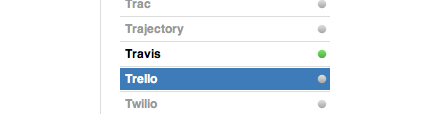
\includegraphics[width=7cm]{img/github_webhook_2.png}
\caption{Github: ''Service hooks'': trello}
\end{figure}

Podešavamo integraciju \href{https://trello.com/board/f18-knowhowerp/50af43adf5c6f78820000223}{\color{blue}{F18 trello table (eng. board), liste ''commits''}}\footnote{detaljnije \url{https://github.com/hernad/agile_dev_env/blob/master/CI.md#f18-knowhwhowerp-trello-integracija}}
\begin{figure}[H]
\centering
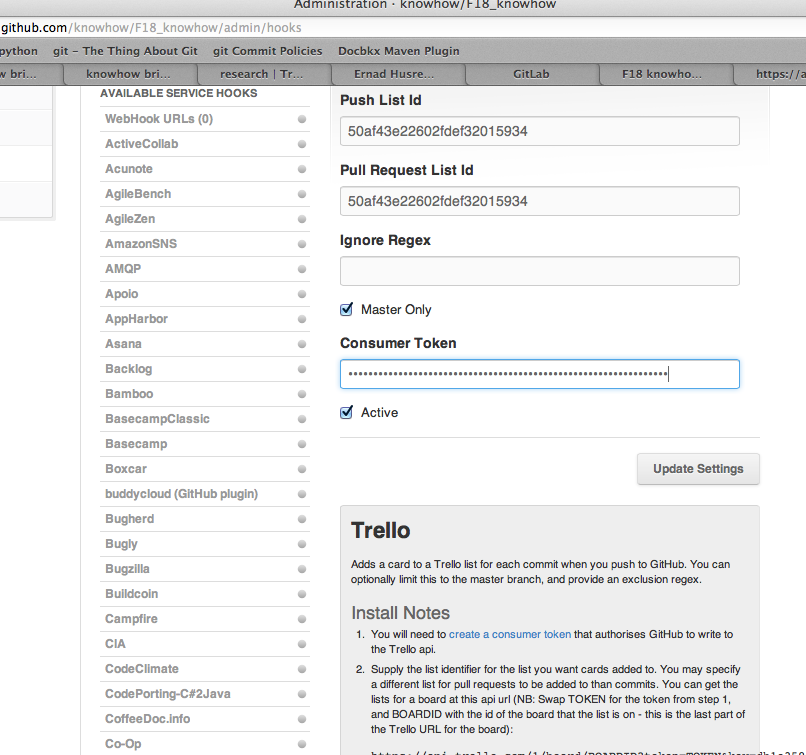
\includegraphics[width=12.5cm]{img/github_webhook_trello_1.png}
\caption{Github: Parametri trello integracije}
\end{figure}

Rezultat integracije je sljedeći:
\begin{figure}[H]
\centering
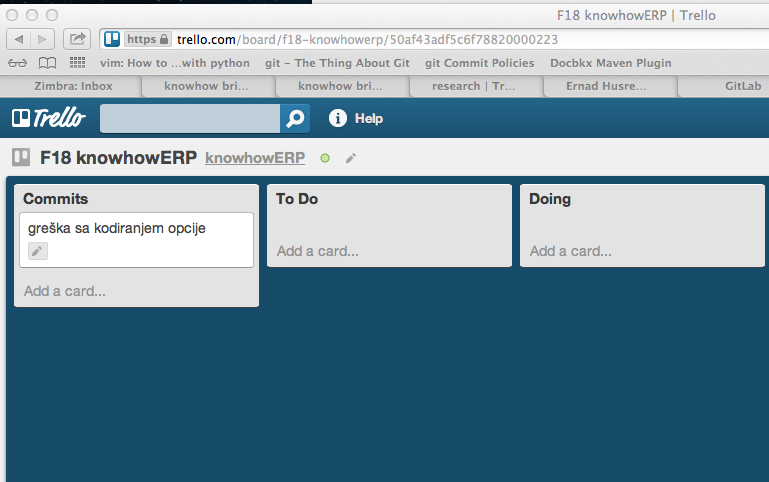
\includegraphics[width=13.5cm]{img/github_webhook_trello_2.png}
\caption{Prikaz ''commit''-a na trello listi ''Commmits''}
\end{figure}

Nakon svakog ''commit''-a na ''F18\_knowhow'' repozitorij, kreira se u listi ''Commits'' trelo kartica (eng. card):

\begin{figure}[H]
\centering
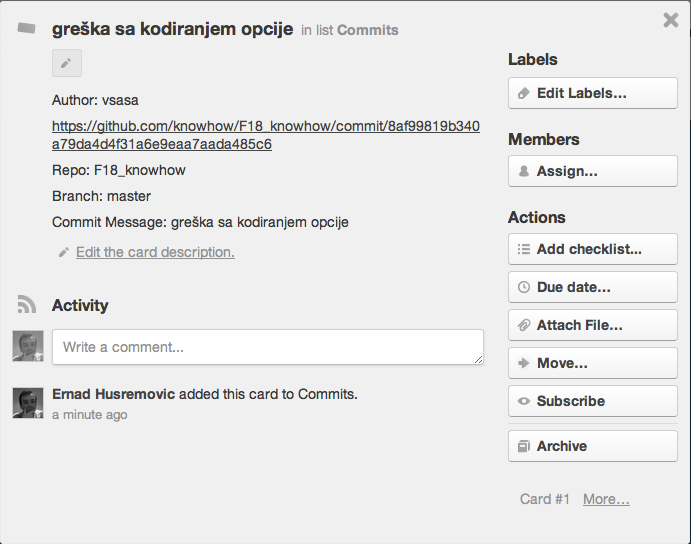
\includegraphics[width=12cm]{img/github_webhook_trello_3.png}
\caption{Git ''commit'' kao ''trello card''}
\end{figure}


\chapter{Ostalo}

\section{Travis \emph{Build matrix}}

U \href{https://github.com/apache/couchdb/blob/master/.travis.yml}{\color{blue}{.travis.yml}} se može definisati više verzija run-time okruženja.

U slučaju "couchdb" projekta radi se o testiranju za više verzija ''erlang'' radnog okruženja. Time se formira matrica buildova za svaku verziju erlang-a:
\begin{figure}[H]
\centering
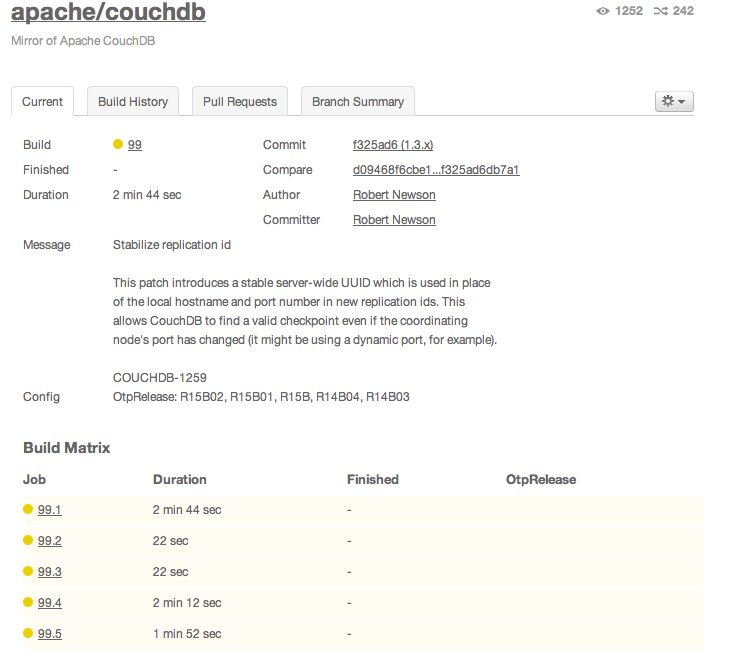
\includegraphics[width=15cm]{img/travis_build_matrix.png}
\caption{Travis build matrica}
\end{figure}

\section{\emph{Travis} je \emph{linux-only} CI}

Ukoliko je projekat ''Windows OS'' orjentisan, travis se ne može koristiti kao CI server, iz jednostavnog razloga što su build sesije isključivo ''ubuntu linux''.

\section{Jenkins CI}

U tom slučaju, jenknins-ci je odlično OSS rješenje \url{http://jenkins-ci.org}. U varijanti ''jenkins''-a je  potrebno je obezbjediti sopstvenu ''build'' infrastrukturu.

Jenkins je jedino (potpuno) rješenje za multiplatformske projekte kao što je slučaj i sa našim primjer projektom materijala - ''F18\_knowhow''.

Jenkins je organizovan java web servlet aplikacija koja se povezuje sa različitim agentima. Tako bi u slučaju ''F18\_knowhow'' trebali bi uspostaviti sljedeću infrastrukturu
\begin{enumerate}
  \item jenkins CI server, ubuntu linux server
  \item jenkins linux agent, ubuntu linux \footnote{funkciju agenta može obavljati i server}
  \item jenkins windows agent
  \item jenkins Mac OS X agent
\end{enumerate}

Agenti obavljaju build operacije po ''instrukcijama'' servera. Korisnik na serveru putem web interfejsa, Webhook-ova prati build proces. Primjetimo da je ''client-agents'' princip jenkinsa sličan ''build matrix'' konceptu ''travis''-a ali omogućava testiranje na različitim operativnim sistemima.


\bibliography{literatura}
\bibliographystyle{fit}

\appendix

\chapter{Priprema F18\_knowhow projekta za \emph{travis build}}
\vspace*{-1.2cm}
Podešenje \emph{travisa} je tražilo značajne operacije, iako su željeni F18 testovi bilo spremni.

Build proces obavlja \href{https://github.com/knowhow/F18_knowhow/blob/master/build_travis.sh}{\color{blue}{build\_travis.sh}} skripta.
Ona obavlja sljedeće:
\begin{enumerate}
  \item instalira harbour sa \emph{google code download} sekcije knowhowERP F18 projekta
  \item kreira bazu i globalne uloge koje test case-ovi koriste
  \item instalira java jod-reports sa google code (eksterni ''dependency'' F18 za generaciju ''ODT'' dokumenata\footer{oasis ''Open document text''format koje koriste openoffice i libreoffice})
  \item build F18\_test
  \item pokreće F18 testove
\end{enumerate}

\section{\emph{Headless} travis podešenja}

Najviše vremena je bilo potrebno da se realizira i testra posljednji korak build procesa pokretanje F18 testova. Razlog za to je što je F18 GUI aplikacija, a travis build sesija na sebi nema ''X Windows'' GUI sistem.

Dobra je stvar da travis nudi rješenje za ovo putem headless konfiguracije\footnote{\url{http://about.travis-ci.org/docs/user/gui-and-headless-browsers}}

\section{Debugiranje \emph{travis} build-a sa \emph{vagrant}-om}

Međutim, i pored svih uputa, bez mogućnosti direktnog testa, u mnogim situacijama ne bi bilo moguće podesiti uspješan \emhp{build  \& test} proces. U te svrhe nam služi činjenica da travis nudi mogućnost da izvršimo \emph{download} \emph{vagrant} sesija koje \emph{travis} koristi\footnote{http://ruby-journal.com/debug-your-failed-test-in-travis-ci}.

\chapter{Ostale bilješke}
\vspace*{-1.2cm}
\section{\emph{Gemnasium} ruby \emph{dependancy management}}

Gemnasium\footnote{\url{https://gemnasium.com/questions}} je samostalan web servis koji se integriše sa github-om. Orjentisam je isključivo na praćenje ruby gem-ova\footnote{Ruby gems \url{http://rubygems.org} je standardizovni sistem za pristup dodatnim ruby bibliotekama i aplikacijama} koji se koriste u sopstevnim projektima. Iako je orjentisam na ''ruby'' projekte, njegov koncept je svakako vrijedan pažnje.

\begin{figure}[H]
\centering
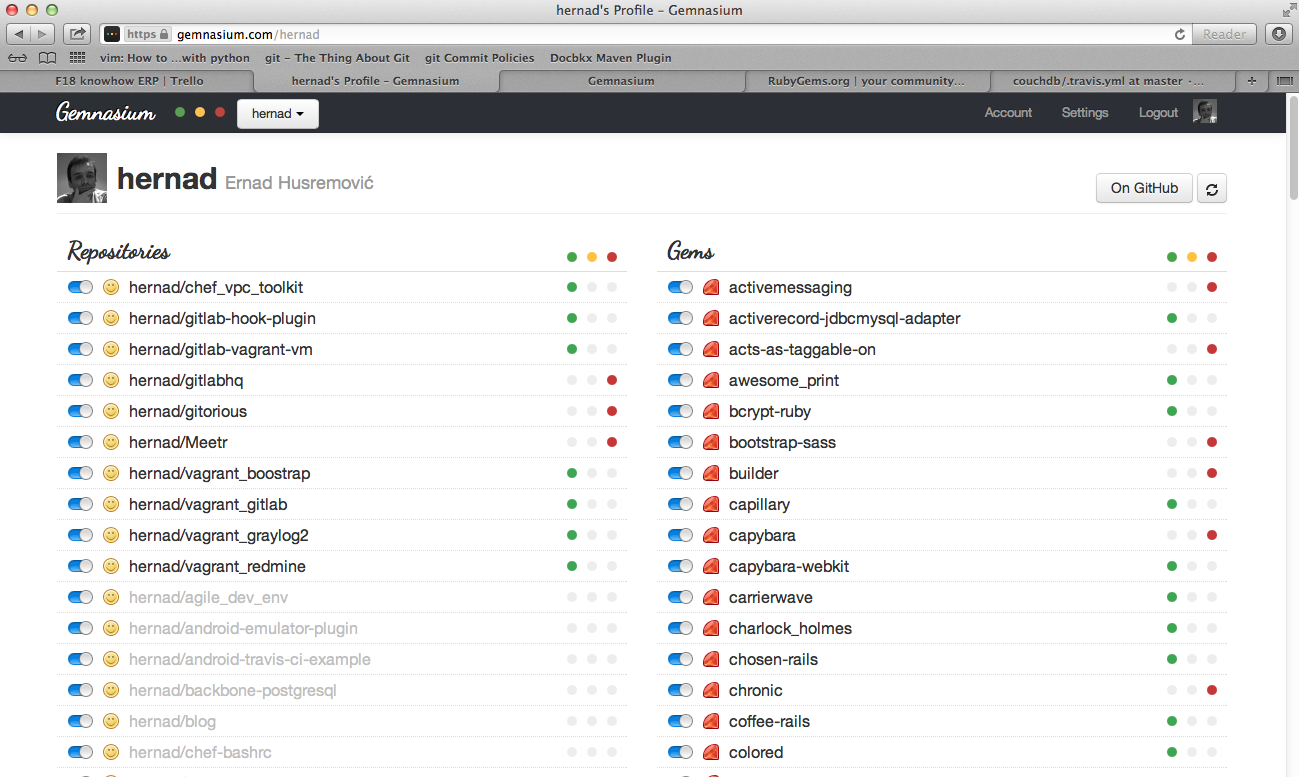
\includegraphics[width=15cm]{img/gemnasium.png}
\caption{Gemnasium za github ''hernad'' korisnički račun}
\end{figure}

\section{Drugi o \emph{travis}-u}

\begin{itemize}
  \item ''Thoughtbot'' \href{http://playbook.thoughtbot.com/tooling-development-process/continuous-integration}{\color{blue}{o travisu}}
\end{itemize}


\end{document}
